\documentclass[aspectratio=43]{beamer}

% ==============================================
% Theme and colors (mimicking the KSU style)
% ==============================================
\usetheme{Madrid}
\usecolortheme{whale}

% Custom orange/KSU gold color for title banners and blocks
\definecolor{ksuorange}{RGB}{245, 166, 35}
\definecolor{ksublack}{RGB}{20,20,20}
\definecolor{titleblue}{RGB}{30,90,170}

% Structure, title, frame title colors
\setbeamercolor{structure}{fg=ksuorange}
\setbeamercolor{frametitle}{bg=ksuorange,fg=white}
\setbeamercolor{title}{bg=ksuorange,fg=white}
\setbeamercolor{author}{fg=black}
\setbeamercolor{date}{fg=black}
\setbeamercolor{institute}{fg=black}
\setbeamercolor{section in head/foot}{bg=ksublack,fg=white}
\setbeamercolor{subsection in head/foot}{bg=ksublack,fg=white}
\setbeamercolor{author in head/foot}{bg=ksublack,fg=white}
\setbeamercolor{title in head/foot}{bg=ksublack,fg=white}
\setbeamercolor{date in head/foot}{bg=ksublack,fg=white}

% Rounded frame title box (matches the rounded orange banner)
\setbeamertemplate{frametitle}[default][leftskip=1ex]
\useinnertheme{rounded}

% Block styling (for theorems/lemmas) in blue like original
\setbeamercolor{block title}{bg=titleblue,fg=white}
\setbeamercolor{block body}{bg=titleblue!8,fg=black}

% Remove navigation symbols
\setbeamertemplate{navigation symbols}{}

% Caption label color (blue, like "Figure:" in original)
\setbeamercolor{caption name}{fg=titleblue}

% ==============================================
% Packages
% ==============================================
\usepackage[utf8]{inputenc}
\usepackage{amsmath, amssymb, amsthm}
\usepackage{graphicx}
\usepackage{booktabs}
\usepackage{array}
\usepackage{xcolor}
\usepackage{hyperref}

% KSU logo in bottom-right of every content slide
\logo{
\includegraphics[width=1cm]{images/ksu_logo.png}}

% ==============================================
% Title page information
% ==============================================
\title[MTA Major Incidents vs. Weather \& Ridership]{Modeling NYC Subway Major Incidents\\Using Weather and Ridership}
\author[Andrew Chincea]{Andrew Chincea}
\institute[KSU]{DATA 3230 -- Data Visualization Final Project\\Kennesaw State University}
\date{April 24, 2026}

% ==============================================
\begin{document}

% ============================================================
% Title slide
% ============================================================
\begin{frame}
  \titlepage
\end{frame}

% ============================================================
% SECTION 1: INTRODUCTION -- Motivation
% ============================================================
\begin{frame}{Motivation}
Every day, millions of New Yorkers rely on the subway, yet \textbf{major incidents} (delays affecting 50 or more trains) regularly disrupt service.

\vspace{0.3cm}
Two natural questions:
\begin{itemize}
  \item How much do \textbf{weather conditions} (snow, rain, heat) drive these disruptions?
  \item Does \textbf{ridership} -- how heavily the system is being used -- explain more of the variation?
\end{itemize}

\vspace{0.3cm}
This project analyzes \textbf{monthly major incidents} from 2015--2024 and builds a statistical model combining both.
\end{frame}

% ============================================================
% Research Questions (rubric item 1)
% ============================================================
\begin{frame}{Research Question}
\begin{block}{Primary Research Question}
Among months between 2020--2024 in the NYC subway system, is the \textbf{monthly count of major incidents} associated with \textbf{monthly total snowfall} and \textbf{monthly subway ridership}, and is the relationship better described as linear or multiplicative?
\end{block}
\small
\begin{itemize}
  \item \textbf{Population:} All calendar months of NYC subway operations, 2020--2024 ($n=60$).
  \item \textbf{Outcome:} Monthly count of major incidents ($\ge 50$ trains delayed).
  \item \textbf{Predictors:} Total monthly snowfall (in.), total monthly ridership (millions), and secondary weather variables.
  \item \textbf{Summary statistics:} Means, SDs, Pearson correlations, regression coefficients, $R^2$, AIC.
  \item \textbf{Analytical method:} \emph{Association between variables} via descriptive correlation and inferential multiple regression.
\end{itemize}
\end{frame}

% ============================================================
% SECTION 2: DATA EXPLANATION (rubric item 2)
% ============================================================
\begin{frame}{Data Sources}
Three public datasets were merged to the monthly level:
\begin{itemize}
  \item \textbf{MTA Incident Data (2015--2024)} -- NY Open Data, one row per major incident with category, line, and timestamp.
  \item \textbf{NOAA Daily Summaries} -- station \texttt{USW00094728} (NYC Central Park): \texttt{TMAX, TMIN, PRCP, SNOW, SNWD}.
  \item \textbf{MTA Subway Hourly Ridership (2020--2024)} -- NY Open Data, boarding counts aggregated to monthly totals (subway mode only).
\end{itemize}

\vspace{0.15cm}
\textbf{Operational definition.} A \emph{major incident} is any incident that delays \textbf{50 or more trains}.

\textbf{Unit of analysis.} One calendar month. Incidents, weather, and ridership are all aggregated to this unit and joined on the month key.
\end{frame}

\begin{frame}{Variables \& Nature}
\footnotesize
\begin{center}
\begin{tabular}{p{3.1cm}p{3.8cm}p{3.3cm}}
\toprule
\textbf{Variable} & \textbf{Type} & \textbf{Role} \\
\midrule
\texttt{total} & count (incidents/month) & outcome \\
\texttt{total\_snow} & continuous (inches) & primary predictor \\
\texttt{ridership\_millions} & continuous (millions) & primary predictor \\
\texttt{avg\_tmax}, \texttt{avg\_tmin} & continuous ($^{\circ}$F) & secondary predictor \\
\texttt{total\_prcp} & continuous (inches) & secondary predictor \\
\texttt{heavy\_precip\_days} & count (PRCP $\ge 0.5$) & engineered feature \\
\texttt{hot\_days} & count (TMAX $\ge 90^{\circ}$F) & engineered feature \\
\texttt{month} & date (year-month) & time key \\
\bottomrule
\end{tabular}
\end{center}

\vspace{0.2cm}
\small All features aggregated to monthly totals or averages so each row represents one month of subway operations in NYC.
\end{frame}

% ============================================================
% DESCRIPTIVE ANALYSIS (part of rubric item 4)
% ============================================================
\begin{frame}{Descriptive Summary (2020--2024, $n=60$ months)}
\small
\begin{center}
\begin{tabular}{lrrrr}
\toprule
\textbf{Variable} & \textbf{Mean} & \textbf{SD} & \textbf{Min} & \textbf{Max} \\
\midrule
Major incidents / month & $\approx 32$ & $\approx 11$ & 5 & 55 \\
Total snow (inches)     & $\approx 2.2$ & $\approx 5.1$ & 0.0 & 25.9 \\
Ridership (millions)    & $\approx 77$ & $\approx 23$ & 20 & 112 \\
Avg.\ TMAX ($^{\circ}$F) & $\approx 64$ & $\approx 16$ & 34 & 89 \\
Heavy precip days       & $\approx 3$ & $\approx 2$ & 0 & 9 \\
\bottomrule
\end{tabular}
\end{center}

\vspace{0.3cm}
\begin{itemize}
  \item Substantial month-to-month variation in both incidents and ridership.
  \item Snowfall is highly skewed -- many months have zero snow, a few have large totals (hence the $\log(\text{snow}+1)$ transformation later).
\end{itemize}
\end{frame}

% ============================================================
% SECTION 3: VISUALIZATIONS (rubric item 3)
% ============================================================
\begin{frame}{Correlation Heatmap (Descriptive)}
\begin{center}
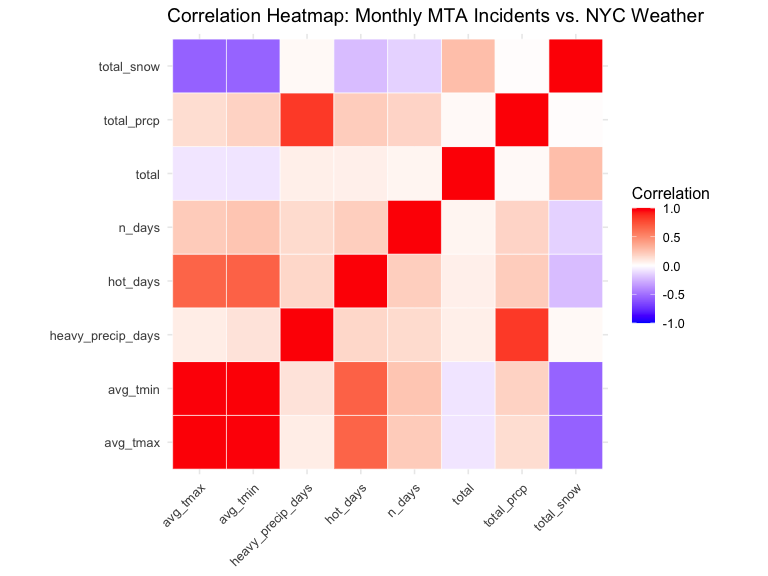
\includegraphics[width=0.54\textwidth]{images/heatmap.png}
\end{center}
\vspace{-0.1cm}
\textbf{Interpretation:} Among weather variables, \textbf{snowfall} has the strongest positive Pearson correlation with monthly incidents; other weather measures show weak associations. This motivates \texttt{total\_snow} as the primary weather predictor.
\end{frame}

\begin{frame}{Visualization: Ridership vs Incidents}
\begin{center}
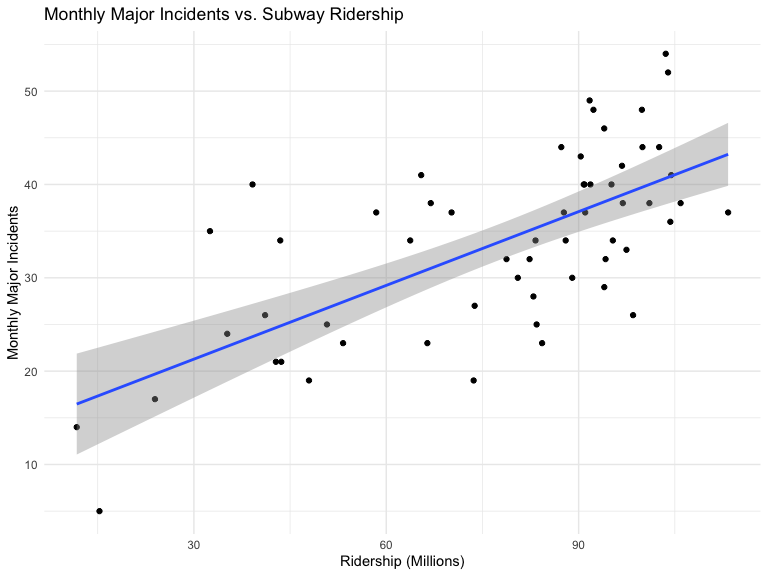
\includegraphics[width=0.62\textwidth]{images/ridership_regression.png}
\end{center}
\vspace{-0.1cm}
\textbf{Interpretation:} Clear positive association -- months with higher ridership tend to have more major incidents, suggesting \emph{exposure} (system usage) is a key driver.
\end{frame}

\begin{frame}{Visualization: Time Series}
\begin{center}
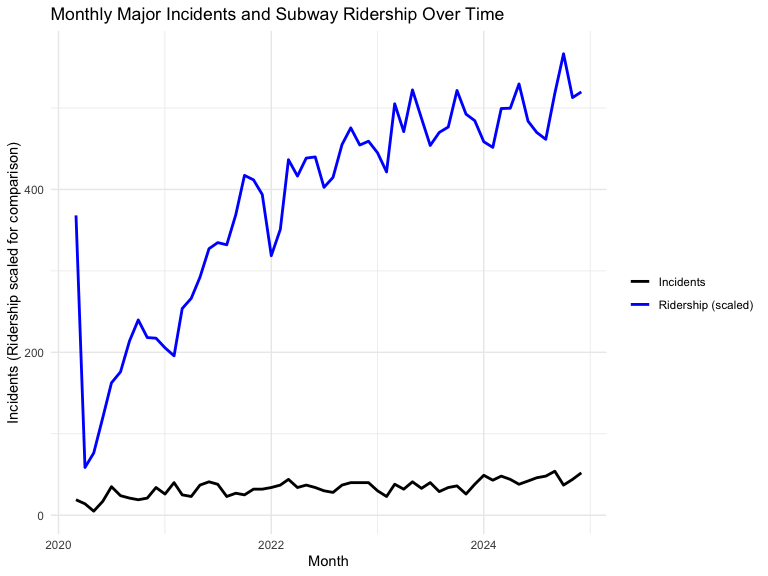
\includegraphics[width=0.70\textwidth]{images/timeseries.png}
\end{center}
\vspace{-0.2cm}
\textbf{Interpretation:} Incidents and ridership track each other over time, including the 2020 COVID-19 collapse and subsequent recovery. This confirms the correlational finding at a temporal level.
\end{frame}

% ============================================================
% SECTION 4: INFERENTIAL ANALYSES (rubric item 4)
% ============================================================
\begin{frame}{Inferential Analysis: Weather-Only Models}
\begin{block}{Candidate Models}
\[
\text{Incidents} = \beta_0 + \beta_1 \text{avg\_tmax} + \beta_2 \text{total\_prcp} + \beta_3 \text{total\_snow} + \varepsilon
\]
\[
\text{Incidents} = \beta_0 + \beta_1 \text{hot\_days} + \beta_2 \text{heavy\_precip\_days} + \beta_3 \text{total\_snow} + \varepsilon
\]
\end{block}

\textbf{Result:}
\begin{itemize}
  \item \texttt{total\_snow} is statistically significant in both ($p < 0.05$).
  \item Other weather terms are \textbf{not} significant.
  \item Overall $R^2$ is low -- weather alone is insufficient.
  \item VIFs all $< 2$; no multicollinearity concern.
\end{itemize}
\end{frame}

\begin{frame}{Inferential Analysis: Snow + Ridership}
\begin{block}{Linear Model (2020--2024, $n=60$)}
\[
\text{Incidents} = \beta_0 + \beta_1\,\text{total\_snow} + \beta_2\,\text{ridership\_millions} + \varepsilon
\]
\end{block}

\textbf{Finding.} Both predictors are statistically significant ($p<0.05$) and jointly explain a large share of variation in monthly incidents.

\vspace{0.1cm}
\textbf{Interpretation.}
\begin{itemize}
  \item Each additional \textbf{million riders} is associated with more incidents, holding snow constant.
  \item Each additional \textbf{inch of snow} is associated with more incidents, holding ridership constant.
  \item Large improvement in $R^2$ over weather-only models.
\end{itemize}
\end{frame}

\begin{frame}{Linear Model Diagnostics}
\begin{columns}[T,onlytextwidth]
  \column{0.5\textwidth}
    \begin{center}
    \small Residuals vs Fitted\\
    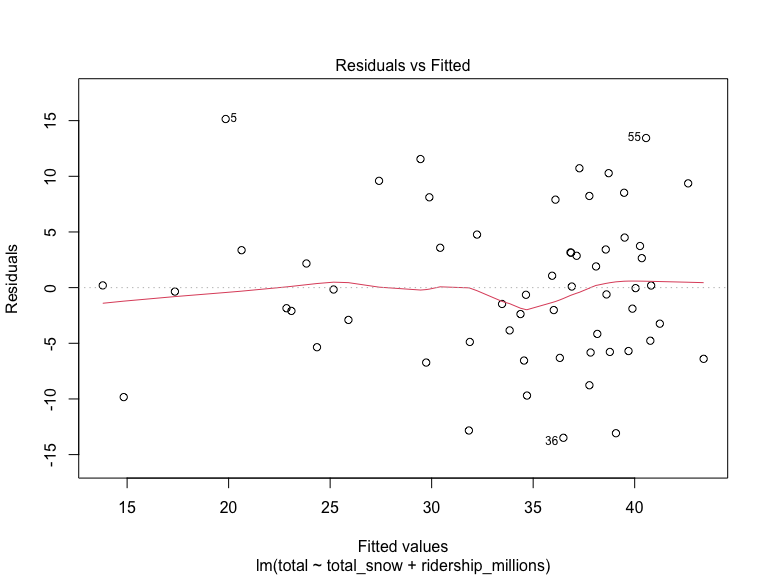
\includegraphics[width=\linewidth]{images/residuals_fitted.png}
    \end{center}
  \column{0.5\textwidth}
    \begin{center}
    \small Normal Q-Q\\
    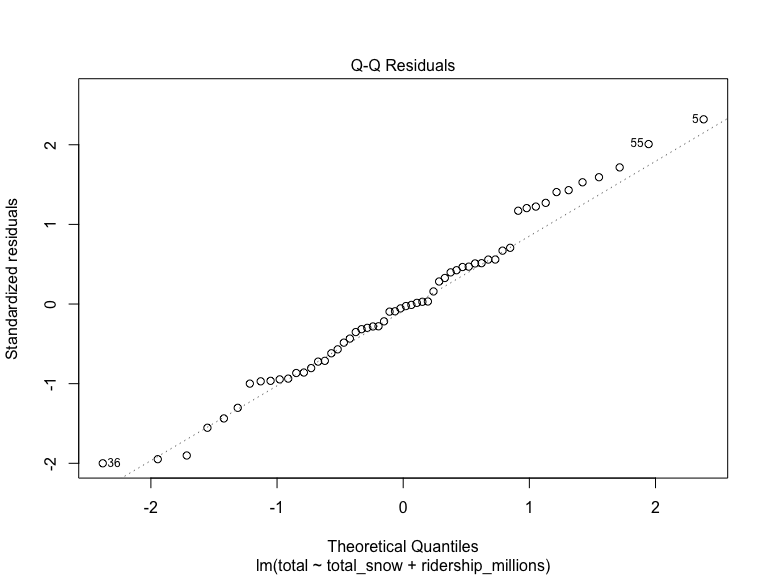
\includegraphics[width=\linewidth]{images/qq_plot.png}
    \end{center}
\end{columns}
\vspace{0.1cm}
\textbf{Interpretation:} Residuals are roughly normal, but mild curvature in the residuals-vs-fitted plot suggests the linear form is not ideal -- motivating a log transformation.
\end{frame}

\begin{frame}{Linear Model Diagnostics (cont.)}
\begin{columns}[T,onlytextwidth]
  \column{0.5\textwidth}
    \begin{center}
    \small Scale-Location\\
    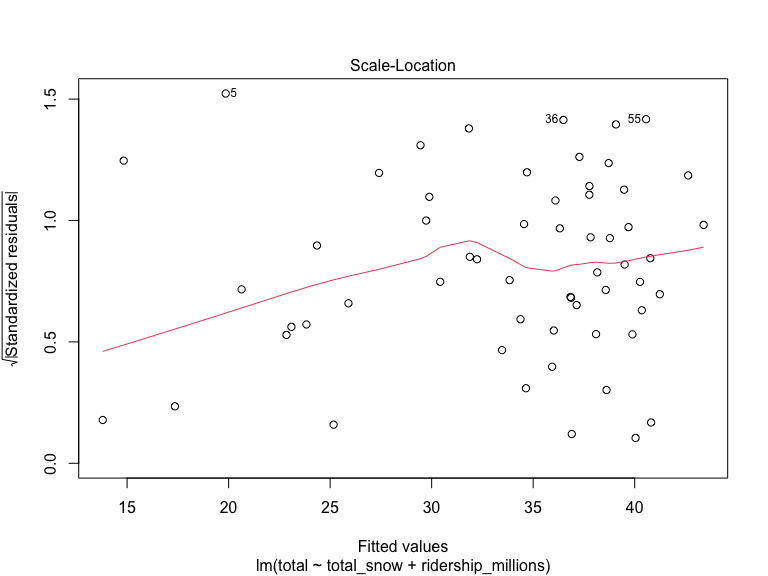
\includegraphics[width=\linewidth]{images/scale_location.png}
    \end{center}
  \column{0.5\textwidth}
    \begin{center}
    \small Residuals vs Leverage\\
    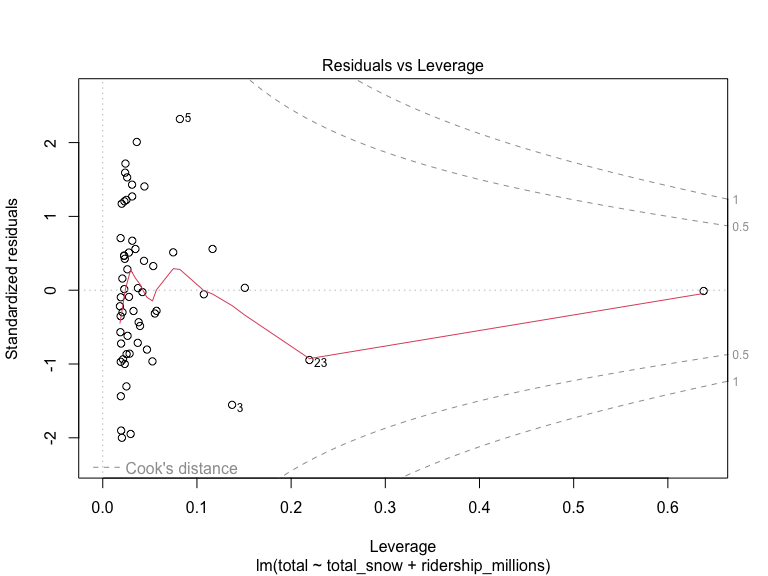
\includegraphics[width=\linewidth]{images/leverage.png}
    \end{center}
\end{columns}
\vspace{0.1cm}
\textbf{Interpretation:} No observations exceed Cook's distance cutoffs, but variance slightly increases with fitted values -- mild heteroscedasticity.
\end{frame}

\begin{frame}{Why a Log-Log Model?}
If the true relationship between incidents, snow, and ridership is \textbf{multiplicative} (e.g., "a 10\% jump in ridership produces a 5\% jump in incidents"), a linear model will systematically mis-fit.

\vspace{0.2cm}
Three candidate specifications compared:
\begin{itemize}
  \item \textbf{Linear:}\quad $y = \beta_0 + \beta_1 s + \beta_2 r + \varepsilon$
  \item \textbf{Log response:}\quad $\log(y) = \beta_0 + \beta_1 s + \beta_2 r + \varepsilon$
  \item \textbf{Log-log:}\quad $\log(y) = \beta_0 + \beta_1 \log(s+1) + \beta_2 \log(r) + \varepsilon$
\end{itemize}

\vspace{0.2cm}
In the log-log model, coefficients are \textbf{elasticities}: a $1\%$ change in the predictor is associated with a $\beta\%$ change in incidents.
\end{frame}

\begin{frame}{Model Comparison via AIC}
\begin{block}{Result}
The \textbf{log-log model has the lowest AIC} of the three candidates.
\end{block}

\vspace{0.1cm}
\begin{center}
\begin{tabular}{lcc}
\toprule
\textbf{Model} & \textbf{df} & \textbf{AIC} \\
\midrule
Linear       & 4 & $392.13$ \\
Log response & 4 & $12.52$  \\
\textbf{Log-log} & \textbf{4} & $\mathbf{5.40}$ \\
\bottomrule
\end{tabular}
\end{center}

\vspace{0.15cm}
\textbf{Interpretation:} The linear model's AIC is nearly 387 units higher than the log-log -- overwhelming evidence in favor of the log-log specification (any $\Delta\text{AIC} > 10$ is considered decisive). The log response alone already improves enormously; adding log-transformed predictors gives the best fit of the three.
\end{frame}

\begin{frame}{Log-Log Regression Coefficients}
\begin{center}
\footnotesize
\begin{tabular}{lrrrl}
\toprule
\textbf{Term} & \textbf{Est.} & \textbf{SE} & \textbf{$t$} & \textbf{$p$-value} \\
\midrule
(Intercept)              & $0.751$ & $0.297$ & $2.53$ & $0.014$\ \hfill * \\
$\log(\text{total\_snow}+1)$ & $0.135$ & $0.045$ & $3.03$ & $0.004$\ \hfill ** \\
$\log(\text{ridership\_millions})$ & $0.626$ & $0.069$ & $9.12$ & $<10^{-11}$\ \hfill *** \\
\bottomrule
\end{tabular}
\end{center}

\vspace{0.2cm}
Residual SE $= 0.243$ on $55$ df.

\vspace{0.2cm}
\textbf{Elasticity interpretation:}
\begin{itemize}
  \item A \textbf{1\% increase in ridership} is associated with a $\approx 0.63\%$ increase in monthly major incidents.
  \item A \textbf{1\% increase in snowfall} (plus one) is associated with a $\approx 0.13\%$ increase in incidents.
  \item Both coefficients are significant; ridership carries far more of the signal.
\end{itemize}
\end{frame}

\begin{frame}{Log-Log: Snowfall vs Incidents}
\begin{center}
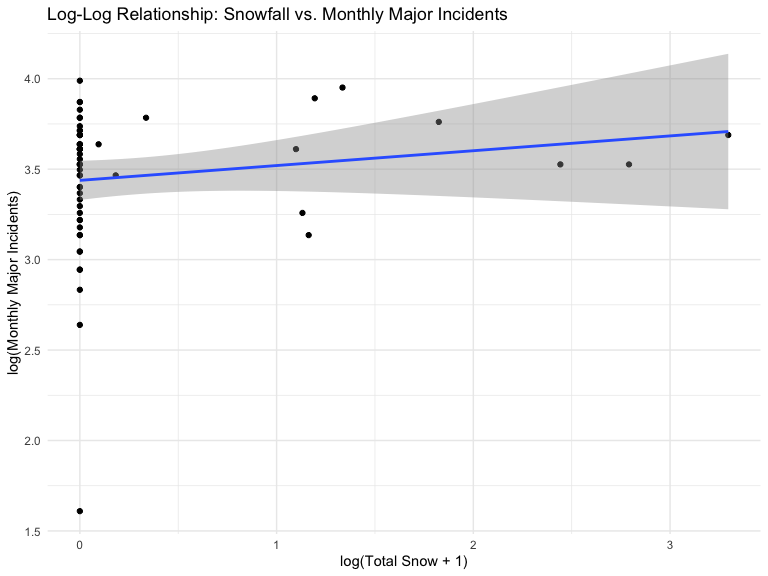
\includegraphics[width=0.70\textwidth]{images/loglog_snow.png}
\end{center}
\vspace{-0.2cm}
On the log scale, the snowfall--incident relationship looks visibly more linear, with a tighter spread around the fit line.
\end{frame}

\begin{frame}{Log-Log: Ridership vs Incidents}
\begin{center}
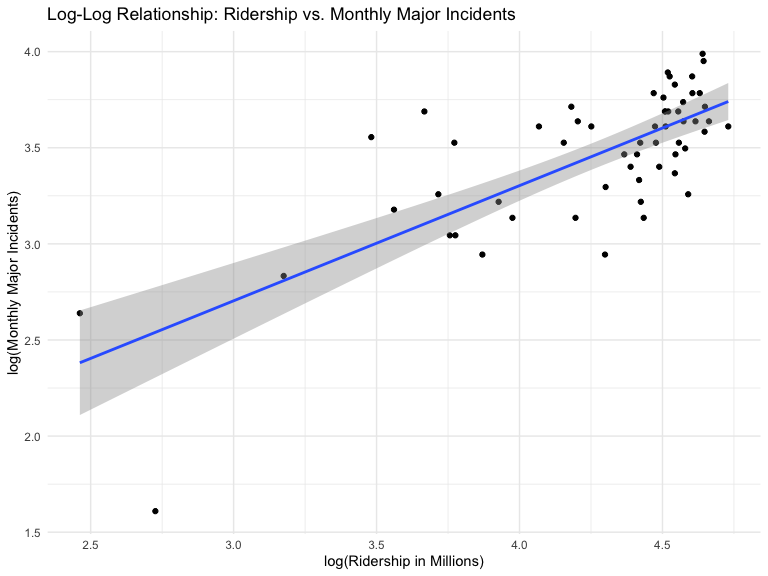
\includegraphics[width=0.70\textwidth]{images/loglog_ridership.png}
\end{center}
\vspace{-0.2cm}
Ridership also shows a cleaner linear pattern after log transformation, consistent with an elasticity-style interpretation.
\end{frame}

\begin{frame}{Actual vs Predicted Incidents}
\begin{center}
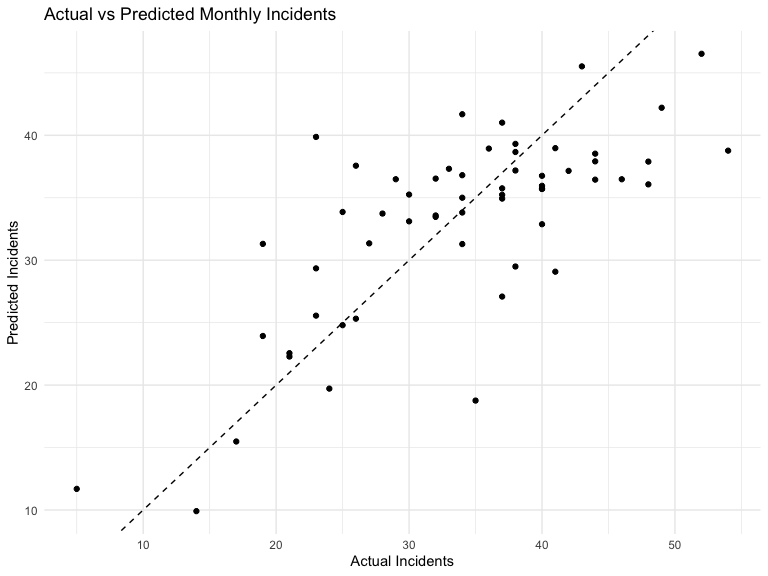
\includegraphics[width=0.65\textwidth]{images/actual_vs_predicted.png}
\end{center}
\vspace{-0.2cm}
Points cluster around the $45^\circ$ reference line: the log-log model's predictions track observed monthly incident counts well.
\end{frame}

\begin{frame}{Actual vs Predicted Over Time}
\begin{center}
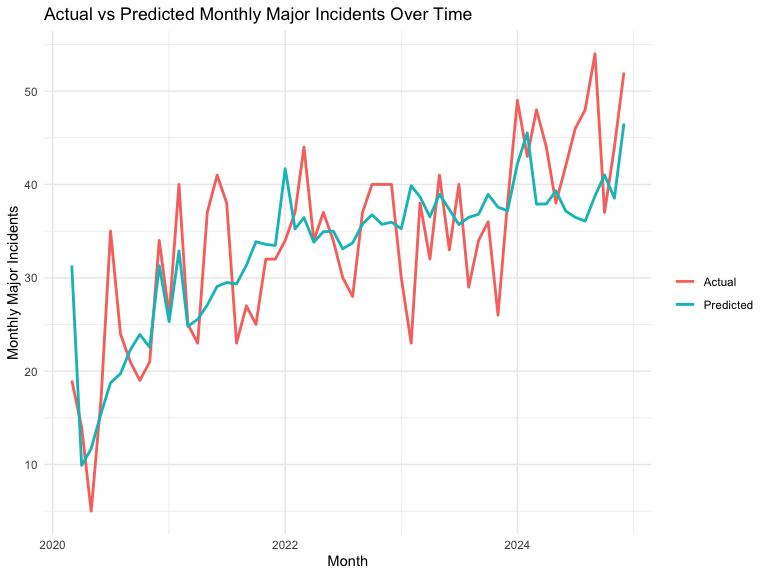
\includegraphics[width=0.72\textwidth]{images/actual_vs_predicted_timeseries.png}
\end{center}
\vspace{-0.2cm}
Predicted series closely follows the observed monthly incident totals, including the 2020 collapse and 2021--2024 recovery.
\end{frame}

\begin{frame}{Log-Log Model Diagnostics}
\begin{columns}[T,onlytextwidth]
  \column{0.5\textwidth}
    \begin{center}
    \small Residuals vs Fitted\\
    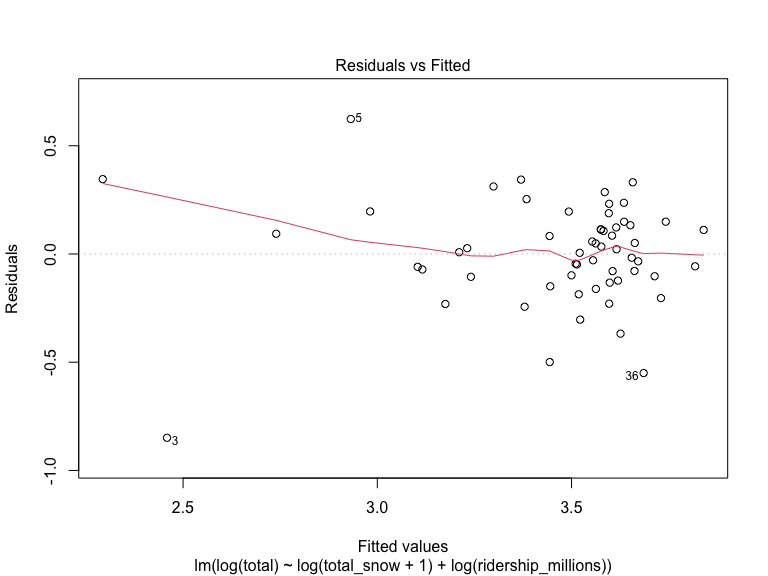
\includegraphics[width=\linewidth]{images/loglog_residuals_fitted.png}
    \end{center}
  \column{0.5\textwidth}
    \begin{center}
    \small Normal Q-Q\\
    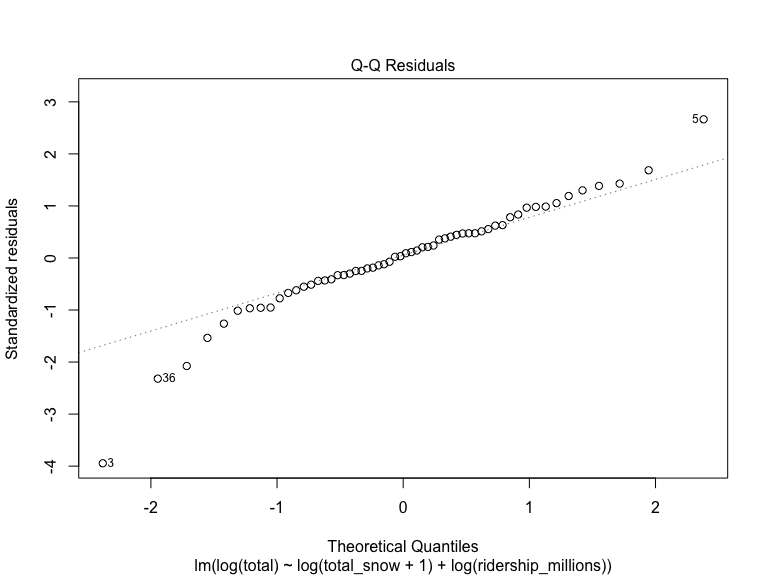
\includegraphics[width=\linewidth]{images/loglog_qq_plot.png}
    \end{center}
\end{columns}
\vspace{0.1cm}
\textbf{Interpretation:} Residuals behave more like iid normal than in the linear model -- tighter, more symmetric, less curvature.
\end{frame}

\begin{frame}{Log-Log Model Diagnostics (cont.)}
\begin{columns}[T,onlytextwidth]
  \column{0.5\textwidth}
    \begin{center}
    \small Scale-Location\\
    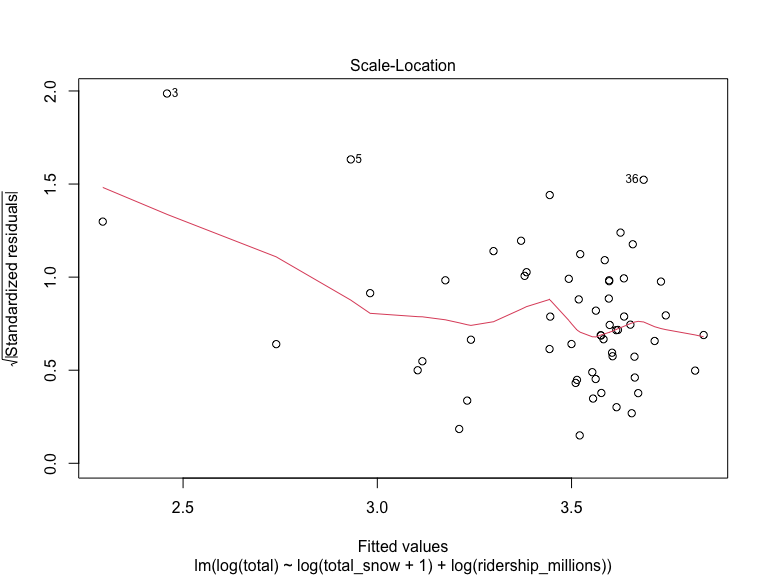
\includegraphics[width=\linewidth]{images/loglog_scale_location.png}
    \end{center}
  \column{0.5\textwidth}
    \begin{center}
    \small Residuals vs Leverage\\
    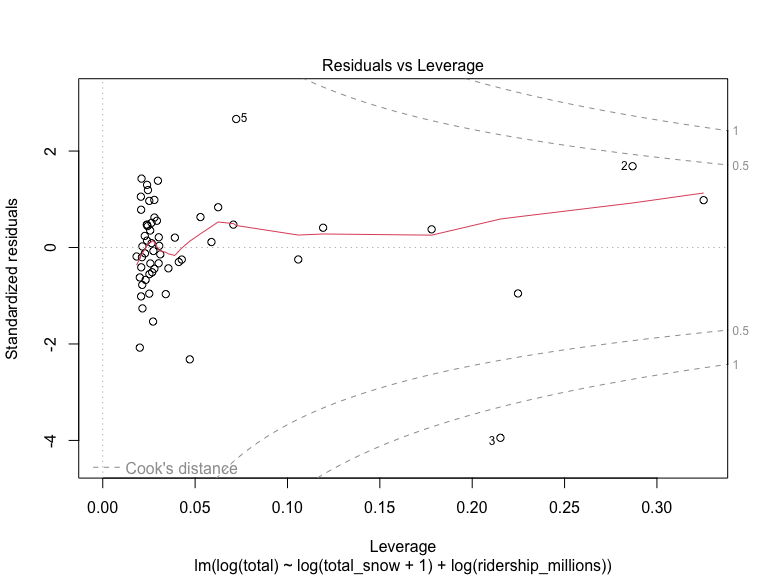
\includegraphics[width=\linewidth]{images/loglog_leverage.png}
    \end{center}
\end{columns}
\vspace{0.1cm}
\textbf{Interpretation:} Variance is noticeably more stable across fitted values, and no points exceed Cook's-distance cutoffs. The log-log specification passes diagnostics more cleanly.
\end{frame}

% ============================================================
% SECTION 5: CONCLUSIONS (rubric item 5)
% ============================================================
\begin{frame}{Answering the Research Question}
\begin{block}{Research Question (restated)}
Is the monthly count of NYC subway major incidents associated with snowfall and ridership, and is the relationship linear or multiplicative?
\end{block}

\vspace{0.2cm}
\textbf{Answer:}
\begin{itemize}
  \item \textbf{Yes} -- both \textbf{snowfall} and \textbf{ridership} are statistically significant predictors of monthly major incidents.
  \item \textbf{Ridership} contributes substantial explanatory power that weather alone cannot; snowfall retains an \emph{independent} effect after controlling for ridership.
  \item The relationship is better described as \textbf{multiplicative}: the log-log model has the lowest AIC and the cleanest residual diagnostics.
\end{itemize}
\end{frame}

\begin{frame}{Limitations}
\begin{itemize}
  \item \textbf{Ridership coverage} -- daily ridership is only publicly available from 2020 onward, restricting the combined model to $n=60$ months.
  \item \textbf{Confounding by COVID-19} -- the early 2020 collapse in both ridership \emph{and} incidents is a dominant signal; relationships may differ in steady-state periods.
  \item \textbf{Aggregation} -- monthly totals smooth over storm-day dynamics; a single 20-inch snowstorm and a month of steady light snow look the same in \texttt{total\_snow}.
  \item \textbf{Single weather station} -- Central Park measurements may not represent borough-level conditions.
  \item \textbf{Association, not causation} -- observational data cannot rule out unmeasured confounders (e.g., capital maintenance cycles, labor actions).
\end{itemize}
\end{frame}

\begin{frame}{Future Work}
\begin{itemize}
  \item Break incidents down by \textbf{category} (signals, track, persons on trackbed) and model each separately.
  \item Add \textbf{lagged} weather effects -- does a storm on day $t$ cause incidents on day $t+1$?
  \item Include \textbf{line-level} ridership instead of system-wide totals.
  \item Try non-linear models (GAMs, random forests) to see whether additional structure remains.
  \item Extend the pre-2020 period once historical ridership becomes available.
\end{itemize}
\end{frame}

% ============================================================
% References
% ============================================================
\begin{frame}{References \& Code}
\small
\textbf{Data:}
\begin{enumerate}
  \item MTA. \textit{Subway Major Incidents 2015--2019} and \textit{2020--2024}. New York State Open Data.
  \item MTA. \textit{Subway Hourly Ridership (2020+)}. New York State Open Data.
  \item NOAA NCEI. \textit{Daily Summaries} -- station \texttt{USW00094728} (NYC Central Park). \\
    \url{https://www.ncei.noaa.gov/access/services/data/v1}
\end{enumerate}

\textbf{Code:} \texttt{FinalVizProject.qmd} (Quarto / R).

\textbf{Tools:} R -- \texttt{dplyr}, \texttt{ggplot2}, \texttt{readr}, \texttt{lubridate}, \texttt{tidyr}, \texttt{httr}, \texttt{car}.
\end{frame}

% ============================================================
% Thank you
% ============================================================
{
\setbeamertemplate{headline}{}
\setbeamertemplate{footline}{}
\begin{frame}[plain]
\vfill
\begin{center}
{\Large Thank you! Any questions?}
\end{center}
\vfill
\end{frame}
}

\end{document}
